%%
%% Dokumentenart
%%
\NeedsTeXFormat{LaTeX2e}
\documentclass[
    a4paper,
    10pt,
    bibliography=totoc,
    twoside,
    openany,
    numbers=noenddot,
    headings=normal,
    DIV=9,
    parskip
    %,draft
]{scrbook}


%%
%% Unterstützung für deutsche Sprache, Umlaute etc.
%%
\usepackage[utf8]{inputenc}
\usepackage[T1]{fontenc}
\usepackage[ngerman]{babel}
\usepackage[babel,german=quotes]{csquotes}


%%
%% Diverse Pakete
%%
\usepackage{scrhack}
\usepackage{graphicx}
\usepackage{verbatim}
\usepackage{tabularx}
\usepackage{subfigure}
\usepackage{url}
\usepackage{color}
\usepackage{amssymb}
\usepackage{amsmath}
\usepackage{amsthm}
\usepackage{setspace}
\usepackage{listings}
\usepackage{colortbl}
%\usepackage{showframe} % Seitenspiegel anzeigen
\usepackage{microtype}
\usepackage{hyperref} % muss letztes Paket in der Liste sein
\usepackage[shadow]{todonotes}
%\usepackage[disable]{todonotes} % keine Kommentare anzeigen
\usepackage{listings}
\usepackage{xcolor}

\lstdefinestyle{sharpc}{language=[Sharp]C, frame=tblr, rulecolor=\color{black!80!black}}


\definecolor{cyan}{HTML}{2B91AF}
\definecolor{comment}{HTML}{008000}
\definecolor{keyword}{HTML}{0000FF}
\definecolor{string}{HTML}{DDDDDD}
\lstset{style=sharpc}
\lstset{basicstyle=\ttfamily\scriptsize,
		keywordstyle=\color{keyword}\ttfamily,
        stringstyle=\color{string}\ttfamily,
		commentstyle=\color{comment}\ttfamily,
		breaklines=true}
\lstset{literate=%
{Ö}{{\"O}}1 
{Ä}{{\"A}}1 
{Ü}{{\"U}}1 
{ß}{{\ss}}2 
{ü}{{\"u}}1 
{ä}{{\"a}}1 
{ö}{{\"o}}1
}
\lstset{emph={%  
    Random, Dictionary, List, Double, Randomizer%
    },emphstyle={\color{cyan}}%
}%

%%
%% hier Namen etc. einsetzen
%%
\newcommand{\fullname}{Rainer Hochdorfer}
\newcommand{\email}{rainer.hochdorfer@uni-ulm.de}
\newcommand{\titel}{Analyse und Bewertung des Laufzeitverhaltens einer Anwendung zur Modalitätsarbitrierung}
\newcommand{\jahr}{2013}
\newcommand{\matnr}{748637}
\newcommand{\gutachterA}{Prof.\ Dr.\ Michael Weber}
\newcommand{\gutachterB}{}
\newcommand{\betreuer}{Frank Honold}
\newcommand{\fakultaet}{Ingenieurwissenschaften\\und Informatik}
%\newcommand{\fakultaet}{Mathematik und\\Wirtschaftswissenschaften}
%\newcommand{\fakultaet}{Naturwissenschaften}
%\newcommand{\fakultaet}{Medizin}
\newcommand{\institut}{Institut für Medieninformatik}
\newcommand{\arbeit}{Bachelorarbeit}
\newcommand{\todor}[1]{\todo[color=green!40]{#1}}
\newcommand{\todof}[1]{\todo[color=yellow!40]{#1}}

%%
%% Setzt Autor und Titel in den Metadaten des erzeugten Dokumentes
%%
\pdfinfo{
    /Author (\fullname)
    /Title (\titel)
    /Producer (pdfeTex 3.14159-1.30.6-2.2)
    /Keywords ()
}
\hypersetup{
    pdftitle=\titel,
    pdfauthor=\fullname,
    pdfsubject={\arbeit},
    pdfproducer={pdfeTex 3.14159-1.30.6-2.2},
    colorlinks=false,
    pdfborder=0 0 0
}


%%
%% Tiefe, bis zu der Überschriften in das Inhaltsverzeichnis kommen
%%
\setcounter{tocdepth}{3}


%%
%% Verhindert überhängende Absatzteile
%%
\clubpenalty10000
\widowpenalty10000
\displaywidowpenalty=10000


%%
%% Einstellungen für Codelistings
%%
\lstset{
    language=Java,
    showstringspaces=false,
    frame=single,
    numbers=left,
    basicstyle=\ttfamily,
    numberstyle=\tiny
}


%%
%% Formatierung des Literaturverzeichnisses
%%
\bibliographystyle{plaindin} % Nummern und alphabetisch sortiert
%\bibliographystyle{alphadin} % Buchstaben und sortiert
%\bibliographystyle{abbrvdin} % Nummern und abgekürzte Namen
%\bibliographystyle{unsrtdin} % Nummern und unsortiert


%%
%% Eigene Makros
%%
\newcommand{\FIXME}[1]{\colorbox{yellow}{\bf FIXME: #1}}


%%
%% Eigene Farben
%%
\definecolor{Gray}{rgb}{0.80784, 0.86667, 0.90196} %dunkelblau
\definecolor{Lightgray}{rgb}{0.9176, 0.95, 0.95686} %hellblau
\definecolor{Akzent}{rgb}{0.6627, 0.63529, 0.55294} %akzentfarbe


%%
%% Liniendicke in Tabellen etc.
%%
\setlength{\arrayrulewidth}{0.1pt}


%%
%% Schriftarten
%%
\renewcommand{\sfdefault}{phv}
\renewcommand{\rmdefault}{phv}
\renewcommand{\ttdefault}{pcr}
\KOMAoptions{DIV=last}


%%
%% Seitenlayout
%%
\pagestyle{headings}


%%
%% Trennungsregeln
%%
\hyphenation{Sil-ben-trenn-ung}


%%
%% Schönere Bullets bei Aufzählungen
%%
\renewcommand{\labelitemi}{$\bullet$}
\renewcommand{\labelitemii}{$\circ$}
\renewcommand{\labelitemiii}{$\cdot$}


%%
%% Beginn des eigentlichen Dokumentes
%%
\begin{document}


%%
%% Vorspann
%%
%%\frontmatter


%%
%% Titelseite
%%
\thispagestyle{empty}
\begin{addmargin*}[4mm]{-32mm}
    % Logo und Wortmarke
    
\includegraphics[height=1.8cm]{images/unilogo_bild}
    \hfill
    
\includegraphics[height=1.8cm]{images/unilogo_wort}
    \vspace*{2.1em}

    % Briefkopf
    \footnotesize
    \textbf{Universität Ulm} \textbar ~89069 Ulm \textbar ~Germany
    \hfill
    \parbox[t]{42mm}{\bfseries Fakultät für\\\fakultaet\\\mdseries\institut}
    \vspace*{2cm}

    % Titel
    \parbox{140mm}{\bfseries \raggedright \huge \titel}

    % Untertitel
    {\arbeit{} an der Universität Ulm}
    \vspace*{4em}

    % Prüfer etc.
    \textbf{Vorgelegt von:}\\\fullname\\\email\\[2em]
    \textbf{Gutachter:}\\\gutachterA\\\gutachterB\\[2em]
    \textbf{Betreuer:}\\\betreuer\\[1.5em]
    \jahr
\end{addmargin*}


%%
%% Impressum
%%



%%
%% Inhaltsverzeichnis
%%
%%\setstretch{1.4}
%%\tableofcontents


%%
%% Hauptteil
%%
%%\mainmatter
\chapter{Motivation}
\chapter{Problemstellung}

\section{Beschreibung}

Im Teilprojekt B3 des Sonderforschungsbereichs Transregio 62 werden aktuell Regeln zur Bewertung der Ausgabegeräte verwendet.
Dies läuft im Moment wie folgt ab:
\begin{figure}[ht]
    \centering
    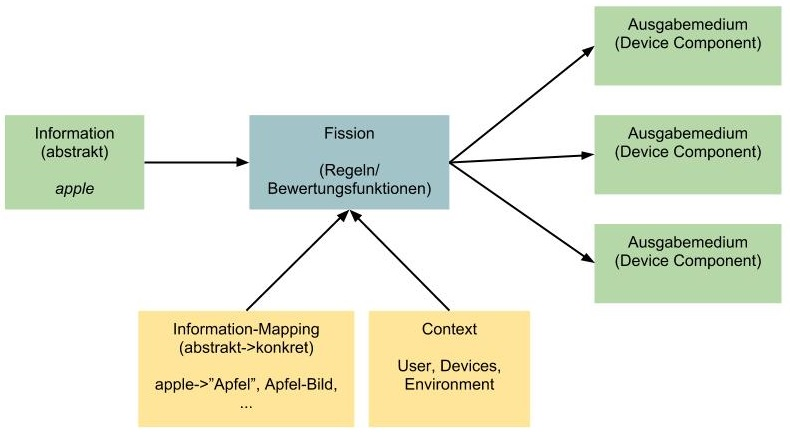
\includegraphics[width=.8\textwidth]{images/FissionUebersicht}
    \caption{\label{fission}Vereinfachte Übersicht der Funktionsweise der Fission}
\end{figure}

 Abstrakte Informationen werden vom Dialog-Manager an die Fission gesendet. Diese abstrakten Informationen werden dann von der Fission wie in Abbildung \ref{fission} zu sehen verarbeitet. Die Fission legt mittels eines Information-Mappings fest, wie die abstrakten Informationen als konkrete Informationen dargestellt werden können. So könnte zum Beispiel die abstrakte Information \emph{apple} sowohl als Text als auch als Bild dargestellt werden. Diese konkreten Daten werden dann im Bezug auf die vorhandenen Kontextinformationen (wie  User-, Environment- oder Device-Context bewertet.
Die Bewertung basiert auf unterschiedlichen Bewertungsfunktionen. Eine Funktion repräsentiert dabei eine gestalterisch bewertete Aussage, z.\,B.: \glqq Es ist sehr gut den akustischen Kanal einzusetzen wenn der Nutzer blind ist.\grqq \ Außerdem besitzt jede Regel einen Funktionswert, der positiv oder negativ sein kann. Alle Regeln werden dann auf alle Kombinationen aus konkreten Informationen und Ausgabemedien(Devices) angewendet. Dabei kann jede Regel mit einer unterschiedlichen Gewichtung in die Bewertung einfließen. Die Gewichtung geht aus dem Kontext hervor.
\linebreak
Dieser Ansatz der Bewertung hat vermutlich exponentielle Laufzeitkomplexität. Davon ausgehend, dass bereits ein weitestgehend optimaler Algorithmus genutzt wird um die Bewertung der Regeln zu berechnen soll dieser Ansatz nun evaluiert werden. Dies dient dazu Aussagen über den Einfluss der Variablen auf die Laufzeit treffen zu können. 

\chapter{Theoretische Analyse}

Wie in der Problemstellung beschrieben, soll aus einem gewissen Set an Informationen zur Verfügung. Aus diesen Informationen soll mit Hilfe eines Algorithmus das optimale Ausgabemedium gewählt werden. Da die eingegebenen Information zum Zeitpunkt der Berechnung feststehen und der Algorithmus auf ein festes Regelwerk zur Berechnung zurückgreift ist dieser deterministisch. Er liefert bei selber Eingabe eine eindeutige Lösung.
Es handelt sich dabei um einen Algorithmus zur Lösung eines Optimierungsproblems.

Zur Lösung von Optimierungsproblemen gibt es verschiedene Kategorien zur Lösung, abhängig vom gewünschten Ergebnis und den zu verwendenden Datenstrukturen. 
\begin{itemize}
	\item Dynamisches Programmieren
	\item Greedy Algorithmen
	\item Optimierung von Baumstrukturen (z.\,B.\ Branch and Bound)
\end{itemize}

\section{Beschreibung des aktuellen Ansatz (Algorithmus)}

\section{Theoretische Bewertung}

\section{Vergleich mit ähnlichen Lösungen}
\chapter{Evaluationsansätze vergleichbarer Systeme}

In diesem Kapitel wird durch Literaturrecherche überprüft wie vergleichbare Systeme evaluiert wurden.

\section{Systeme zur Modalitätsarbitrierung}

Es wurden bereits einige Ansätze zur Evaluation von Systemen zur Modalitätsarbitrierung versucht. Dabei wird im allgemeinen versucht \todor{Quelle der Spanier} zu überprüfen wie adaptiv ein System ist. Das bedeutet es werden die Ergebnisse qualitativ überprüft. Keiner der Ansätze überprüfte dabei das Laufzeitverhalten des Algorithmus. Darum werden im folgenden Abschnitt Evaluationsansätze für vergleichbare Algorithmen betrachtet.

\section{Evaluationsansätze vergleichbarer Algorithmen}

Wie im vorigen Abschnitt beschrieben existieren bisher keine Evaluationsansätze für die Analyse des Laufzeitverhaltens eines Systems zur Modalitätsarbitrierung. Aus diesem Grund sollen in diesem Teil nun vergleichbare Algorithmen betrachtet werden.
\chapter{Evaluation}

Das Ziel der Evaluation ist die Performance des Fissions-Algorithmus zu messen, welcher die Bewertungsfunktionen für verschiedene Dialog-Outputs berechnet. Wie in der Theoretischen Betrachtung festgestellt sind dabei folgende unabhängigen Variablensets zu beachten: \emph{Personmodel}, \emph{Surroundingsmodel}, \emph{DistanceRelations}, die \emph{Device}- und \emph{Componentmodel} Permutationen, \emph{Rules} und der jeweilige \emph{DialogOutput}. Zudem gilt es die Hardwarekonfiguration des Testsystems zu beachten.
Abhängige Variable ist die Zeit, die der Algorithmus zur Berechnung benötigt.

\section{Entwicklung des Tools zur Evaluation}
Um das Evaluationsvorhaben durchzuführen wird ein zusätzliches Tool entwickelt. Es hat insbesondere drei Aufgaben: Erzeugen von generischen Testdaten (unabhängige Variablen), Versand der Daten als Semaine-Nachrichten an die Fission und das Logging der Testergebnisse (abhängige Variablen).

\subsection{Generische Testdaten}
Bei der generischen Erzeugung der Testdaten gelten spezielle Anforderungen. Mit der Klasse \emph{Random}, die durch das .Net Framework zur Verfügung gestellt können Zufallszahlen erzeugt werden. Jedoch bietet diese Klasse keine Funktionen an um Wahrscheinlichkeitsverteilungen zu erzeugen. Für die Erzeugung dieser Zufallswerte \todor{auf Zufallswerte eingehen} wurde die statische Klasse \emph{Randomizer} erstellt. Diese bietet verschiedene Methoden an um die generischen Testdaten zu erzeugen.
\subsubsection{Zufällige, gleichverteilte Wahrscheinlichkeitswerte}
Eine dieser Anforderungen war es, für beliebig viele Entitäten eine Wahrscheinlichkeitsverteilung zu erzeugen, die in Summe eine vorgegebene Gesamtwahrscheinlichkeit ergibt. Die Einzelwerte sollen hierbei jedoch zufällig gleichverteilt und \emph{nicht} normalverteilt sein. Eine mathematische Lösung für dieses Problem bietet folgender Ansatz\footnote{http://www.matheboard.de/archive/501805/thread.html, 14.11.2013}:
\begin{enumerate}
\item Erzeuge \( n \)  verschiedene Zufallszahlen \(z_{i}, i = 1...n \) mit \(z_{i} \in \mathbb{R}^+ \) 
\item Summiere über alle Zufallszahlen: \( z:= \sum_{i=1}^{n} z_{i}\)
\item Teile die gewünschte Summe der Zufallszahlen \( s \)  durch die Summe der \\Zufallszahlen \( z \): \( \frac{s}{z} = m\)
\item Multipliziere alle Zufallszahlen \( z_{1} ... z_{n} \) mit dem Faktor \( m \) und erhalte die gewünschten Zufallszahlen \( y_{1} ... y_{n} \) mit \( s = \sum_{i=1}^{n} y_{i}\) mit \(y_{i} = m * z_{i} \)
\end{enumerate}
Diese Schritte sind im Algorithmus (Listing \ref{RandomDistribution}) umgesetzt. Der Methode müssen ein \emph{Random}-Objekt, die gewünschte Summe der Zufallszahlen (bei Wahrscheinlichkeitsverteilung z.\,B.\ 1 (=100\%)) und die Anzahl der Werte übergeben werden. Das \emph{Random}-Objekt wird an die Methode übergeben, da bei mehrfachem Aufruf der Methode dasselbe Objekt verwendet werden sollte, um eine breite Streuung der Zufallszahlen zu erhalten.

\lstset{caption={Gleichverteilte Wahrscheinlichkeitsverteilung für beliebig viele Werte},label=RandomDistribution}
\begin{lstlisting}
public static List<Double> RandomDistribution(Random rnd, Double sum, Int32 count)
{
    // Liste für die erstellten Werte (Rückgabewert)
    List<Double> randomValues = new List<Double>();
    // Summe der Zufallszahlen
    Double sumZ = 0;

    for (Int32 i = 0; i < count; i++)
    {
        Double randomValue = rnd.NextDouble();
        // Erzeuge die gewünschte Anzahl Zufallswärte
        randomValues.Add(randomValue);
        // Berechne Summe z der erzeugten Zufallswerte
        sumZ += randomValue;
    }

    // Sei sum = x. Teile x/z = m.
    if (sumZ <= 0)
    {
        // Nicht durch 0 teilen, Wert sollte positiv sein!
        return null;
    }
    Double multiply = sum / sumZ;

    // Multipliziere alle Zufallszahlen mit m.
    for (Int32 i = 0; i < count; i++)
    {
        randomValues[i] = randomValues[i] * multiply;
    }

    return randomValues;
}
\end{lstlisting}


\subsubsection{Zufällige Intgerwerte mit gleichverteilten Wahrscheinlichkeitswerten}
Eine weitere Anforderung ist die zufällige Generierung von beliebig, jedoch nur einmal auftretenden Integer-Werten innerhalb eines bestimmten Intervalls. Diese wiederum müssen mit einer Wahrscheinlichkeitsverteilung versehen sein. So soll z.\,B.\ auf einer Skala von eins bis zehn, n zufällige Werte gewählt und mit einer Wahrscheinlichkeit belegt werden. Die Summe der n Wahrscheinlichkeitswerte soll eins ergeben (etwa: 3=0,2; 4=0,1; 6=0,4; 9=0,3). Der in Listing \ref{IntAndProbabilityDistribuion} dargestellte Algorithmus erzeugt eine zufällige Anzahl beliebiger jedoch distinkter Integer-Werte in einem vorgegebenen Zahlenbereich [min, max]. Diesen Zahlen wiederum wird dann mit der im vorangegangenen Abschnitt beschriebenen Methode eine Wahrscheinlichkeitsverteilung zugeordnet. Diese Zuordnung wird in einem \emph{Dictionary<int,double>} gespeichert und zurückgegeben.
\lstset{caption={Gleichverteilte Wahrscheinlichkeitsverteilung für beliebige Integerwerte},label=IntAndProbabilityDistribuion}
\begin{lstlisting}
public static Dictionary<int, double> IntAndProbabilityDistribuion( Random rnd,  int min, int max, double sum) {

	// Rückgabewert
    Dictionary<int, double> distribution = new Dictionary<int, double>();

    List<int> values = new List<int>();
    // Erzeuge eine bestimmt Anzahl an Werten
    int countValues = Randomizer.GenerateRandomNumber(min, max);
    for (int i = 0; i<countValues; i++)
    {
        int newValue;
        do {
            newValue = Randomizer.GenerateRandomNumber(min, max);
        }
        while (values.Contains(newValue));
        // Füge einzigartige Zahl hinzu
        values.Add(newValue);
    }
    // Erzeuge Wahrscheinlichkeiten
    List<double> valueProbabilities = Randomizer.RandomDistribution(rnd, sum, countValues);
    // Füge Werte in Model ein
    for (int i = 0; i < countValues; i++)
    {
        distribution.Add(values[i], valueProbabilities[i]);
    }

    return distribution;
}
\end{lstlisting}




\subsection{Versand der Nachrichten}
XML Nachrichten werden mit Hilfe der Klassen erzeugt, welche generische Testdaten erzeugen. Diese werden dann mit \emph{Semaine Sender Components} an die Middleware und somit an die Fission verschickt.
An dieser Stelle ist dies Beispielhaft für das PersonModel beschrieben:

\lstset{caption={Semaine Copmponent PersonModelSender},label=PersonModelSender}
\begin{lstlisting}
class PersonModelSender: Component
{
    // Die Sender und Receiver
    private XMLSender _personModelSender;
    private Receiver _requestReceiver;

    // Konstruktor
    public PersonModelSender()
        : base("B3.Budgie.PersonModelSender")
    {
        //Person Model request Receiver
        _requestReceiver = new Receiver("semaine.data.user.request");
        _receivers.AddLast(_requestReceiver);
        // Person Model Sender
        _personModelSender = new XMLSender("semaine.data.user", "XML", this.GetType().Name);
        _senders.AddLast(_personModelSender);
    }

    // Reagiere auf Requests
    protected override void React(SEMAINEMessage message)
    {
        if (message.Text.Equals("UPDATE", StringComparison.OrdinalIgnoreCase)) {
            GenericPersonModel person = new GenericPersonModel("person_id");
            XmlDocument doc = person.Person.XmlRepresentation;
            _personModelSender.SendXML(doc, _meta.CurrentTime);
        }
    } 
}
\end{lstlisting}






\section{Durchführung}



\chapter{Auswertung und Diskussion}

\section{Zusammenfassung}

\section{Diskussion}

\section{Evtl. Verbesserungsansätze}
% hier weitere Kapitel einbinden


%%
%% Anhänge
%%
%%\appendix
%%\chapter{Quelltexte}

In diesem Anhang sind einige wichtige Quelltexte aufgeführt.

\begin{lstlisting}
public class Hello {
    public static void main(String[] args) {
        System.out.println("Hello World");
    }
}
\end{lstlisting}



%%
%% Nachspann
%%
%%\backmatter


%%
%% Literaturverzeichnis
%%
%%\bibliography{bibliography}


%%
%% Versicherung
%%
%%\cleardoublepage
%%\thispagestyle{empty}

%%Name: \fullname \hfill Matrikelnummer: \matnr \vspace{2cm}

%%\minisec{Erklärung}

%%Ich erkläre, dass ich die Arbeit selbständig verfasst und keine anderen als die angegebenen Quellen und Hilfsmittel verwendet habe.\vspace{2cm}

%%Ulm, den \dotfill

%%\hfill {\footnotesize \fullname}
\end{document}
